\subsection{Modelo de iOS}
\begin{frame}
 \begin{center}
  \LARGE Modelo de iOS
 \end{center}
\end{frame}
\begin{frame}
 \frametitle{Modelo de iOS}
 \begin{figure}[tH]
  \begin{subfigure}{0.7\linewidth}
   \begin{itemize}
    \item iOS es un sistema operativo para dispositivos móviles de la multinacional Apple Inc. diseñado para ser
seguro. \pause
    \item Las principales características de seguridad no son configurables y vienen habilitadas por defecto. \pause
   \end{itemize}
  \end{subfigure}
  \begin{subfigure}{0.25\linewidth}\pause
    \centering
    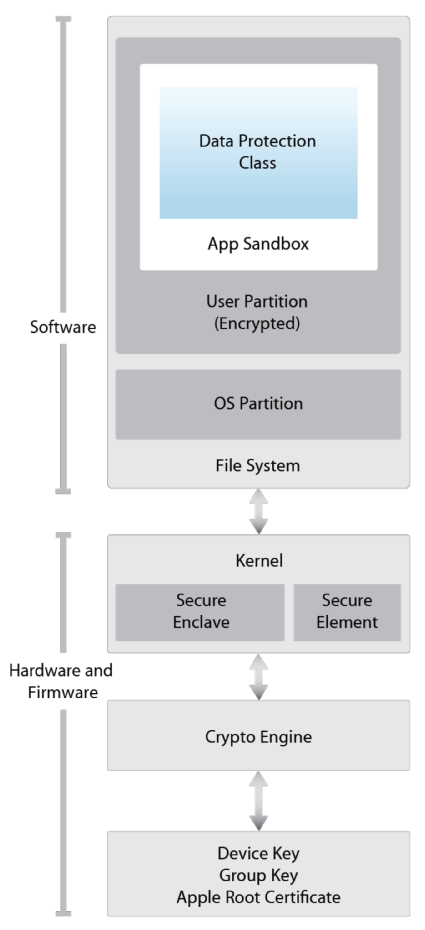
\includegraphics[width=\linewidth]{ios_security_architecture}
  \end{subfigure}
  \caption{Entorno seguro de iOS.}
\end{figure}
\end{frame}
\begin{frame}
 \frametitle{Modelo de iOS}
 \begin{itemize}
  \item Las aplicaciones pueden solicitar un permiso solamente mientras se esté ejecutando. \pause
 \end{itemize}
 \begin{figure}[hbtp]
    \centering
    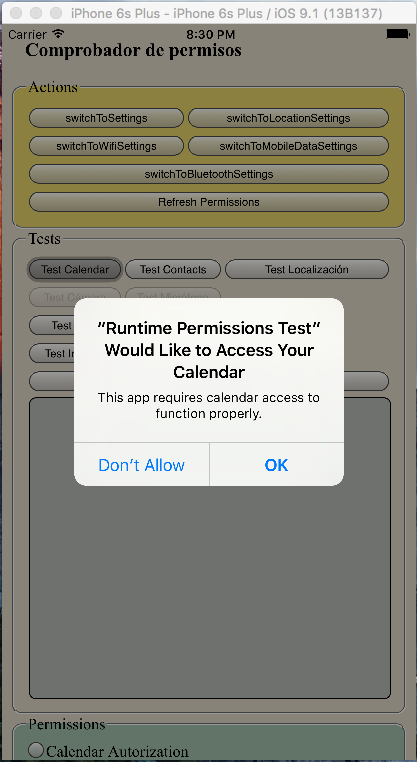
\includegraphics[width=.25\linewidth]{calendar_request_ios}
    \caption{Control de privacidad de iOS 9.}
 \end{figure}
\end{frame}
